\begin{frame}[c]{Datentransfer}
	\hspace{-0.3cm}
	\begin{tikzpicture}[scale=0.7, transform shape]
		\node (A) at (0,0) {};
		\draw (A) circle (1.5) [path picture={ 
				\node at (path picture bounding box.center){
					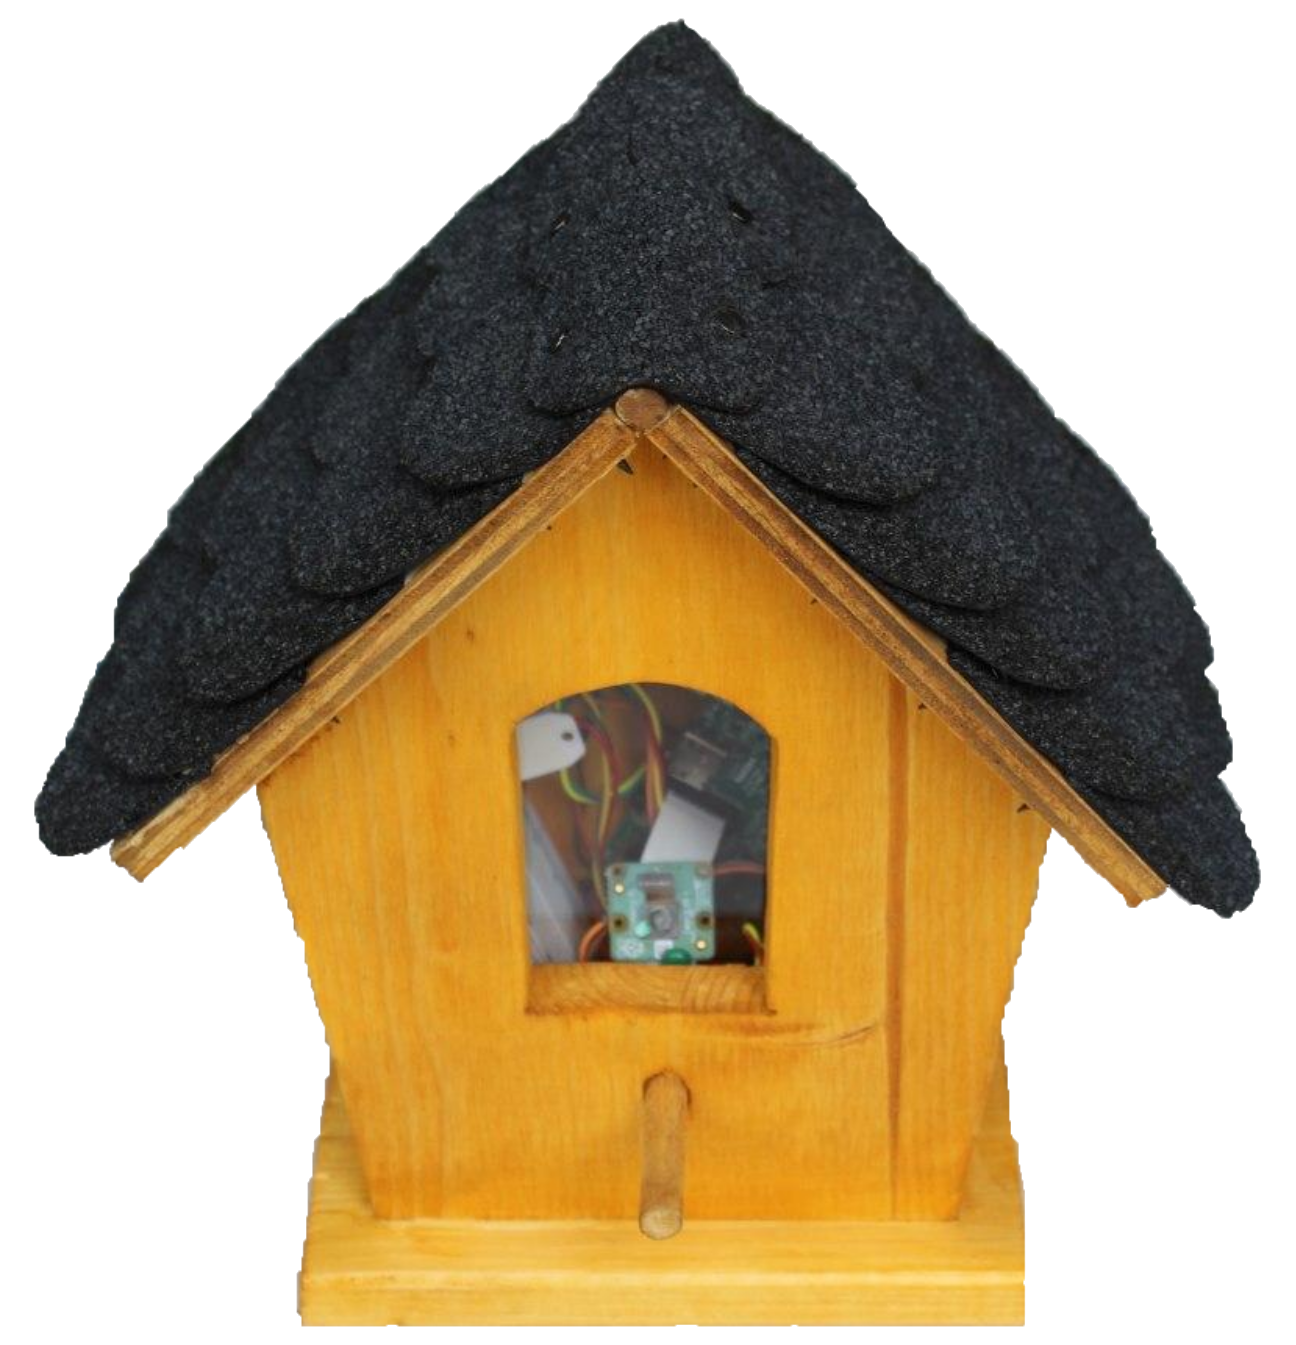
\includegraphics[height=2.6cm]{picture/wetterstation.png}};
			}, line width=1];

		\draw (A)++(2.25,-4) [fill=black!10] rectangle ++(3.5,8.5);
		\node (B) at (4, 4) {Datentransfer};
		\draw (A)++(4,2) circle (1.3) [path picture={ 
				\node at (path picture bounding box.center){
					
\includegraphics[width=2.6cm]{picture/mariadb.png}};
			}, line width=1];
		\draw (A)++(4,-2) circle (1.3) [path picture={ 
				\node at (path picture bounding box.center){
					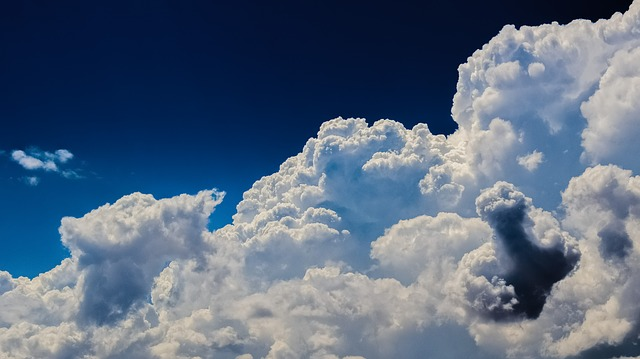
\includegraphics[height=2.6cm]{picture/clouds.jpg}};
			}, line width=1];

		\draw (A)++(8,0) circle (1.3) [path picture={ 
				\node at (path picture bounding box.center){
					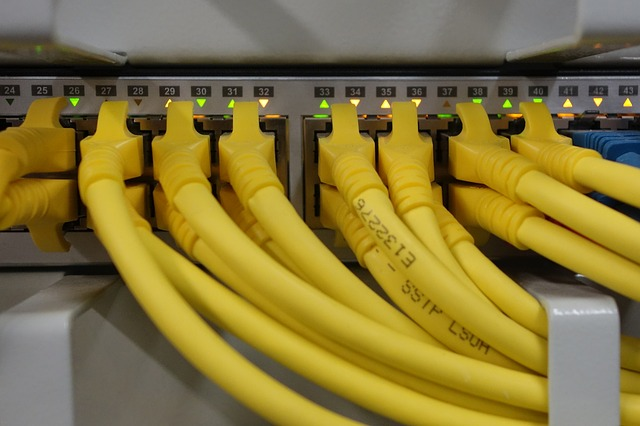
\includegraphics[height=2.6cm]{picture/network.jpg}};
			}, line width=1];

		\draw (A)++(10.50,-4) [fill=black!10] rectangle ++(3.5,8.5);
		\node (D) at (12.25, 4) {Auswertung};
		\draw (A)++(11,0.75) rectangle ++(2.5,2.5) [path picture={ 
				\node at (path picture bounding box.center){
					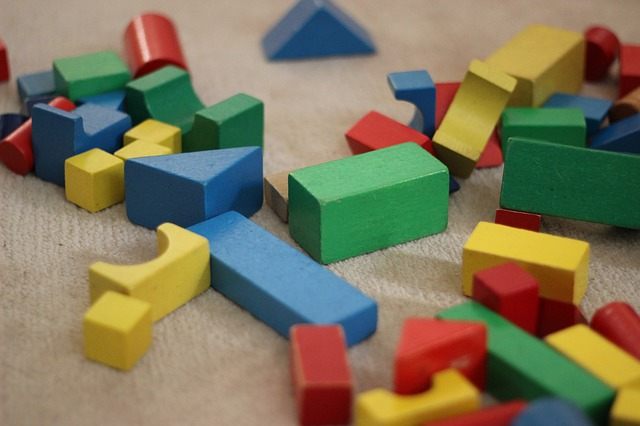
\includegraphics[height=2.5cm]{picture/building_blocks.jpg}};
			}, line width=1];
		\draw (A)++(11,-3.25) rectangle ++(2.5,2.5) [path picture={ 
				\node at (path picture bounding box.center){
					
\includegraphics[height=2.0cm]{picture/telegram.png}};
			}, line width=1];

	\end{tikzpicture}
\end{frame}
